\section{Evaluation of Interest flooding mitigation methods}
\label{sec:evaluation}

% List all possible parameters, say clearly which ones we vary, and which ones we do not, along with explanations.

% Metrics that we will consider in our evaluation (Satisfaction rate for good clients, Link utilization near producers, 

% alex: what's a point of latency?  it would matter only for queueing method and we not really pushing this method
% Latency for good clients, good versus bad interests as a function of time

In this section present an in-depth study, aiming to explore quality and effectiveness of the designed Interest flooding attack mitigation methods.
Our study is based on simulations performed with the help of open-source ndnSIM~\cite{ndnsim} package, which implements NDN protocol stack for NS-3 network simulator.\footnote{\url{http://www.nsnam.org/}}

% why we chose small scale topology
% what point we wanted to show we small scale
% what points we wanted to verify with larger-scale internet like topology

% Metrics
% not sure if i already explained that. our essential qualitative metric is .  
% To quantify the effectiveness of the mitigation mechanism this  metric we use satisfaction percentages of user Interests.
Quality of the attack mitigation methods directly corresponds to the quality of service for the legitimate users during an ongoing attack, which in NDN network can be quantified through percentage of satisfied Interest.
For example, if the network implements a mitigation method $X$ and under the attack majority of user-expressed Interests are getting satisfied, then the method $X$ can be seen as highly effective.
At the same time, if only a small percentage of the expressed Interest are getting satisfied during the attack, the method $X$ can be called ineffective. 

% Traffic pattern
In our experiments we made a simplistic assumption that both legitimate users and adversaries express Interests with constant average rates with randomized (uniform distribution) time gaps between each two consecutive Interests.
% Alex: not sure how to argue about the traffic pattern
Although this pattern is not truly realistic, it gives us a good statistical mix of traffic from all network users without excessive network buffering.

In addition to that, in each run of the simulation we ensure that all Interests expressed by the legitimate users during a no-attack period are satisfied.
For simplicity and without losing any generality, we also equalized the average rates with which the legitimate users express Interests.
At the same time, the attackers are sending junk Interests as much as they can get through (remember, that Interest limits will not allow real flooding of Intersests in all of the designed mitigation algorithms).

% Fixed parameters
The \emph{Delay} and \emph{Data size} parameters for the Interest limits calculation (1) were set to fixed values for every node in the simulated topology.
In particular, for the small-scale experiments we set Delay to 80~ms and for the large-scale experiments we used the value 330~ms (the order of the largest RTT).
Data size parameter was set to 1100~bytes for all simulation runs and topologies.

\subsection{Small-scale evaluations}
\label{sec:small-scale}

% Topology description
%To assess baseline quality of the designed Interest flooding attack mitigation methods, we evaluated them first using a %simplistic small-scale binary tree topology 
In Fig.~\ref{fig:small-scale}, we depict the binary-tree topology that we use for our initial experiments.
Legitimate users as well as attackers were placed on leaf nodes (red nodes) as show in the figure. There are 16 end users (both legitimate and attackers) in this topology, each expressing Interests that are routed towards a single data producer placed at the root of the tree.  Each link in this topology is assigned a bandwidth of 10~Mbps and a randomized propagation delay ranging from 1 to 10 ms. 

% Alex: should we mention that?
%The main reason to chose a binary tree topology was that it represents one of the worst cases to defend against flooding DDoS %attacks.
%That is, sharing of the network links exponentially increases as decreasing level of the binary tree.

\begin{figure}[]
  \centering
  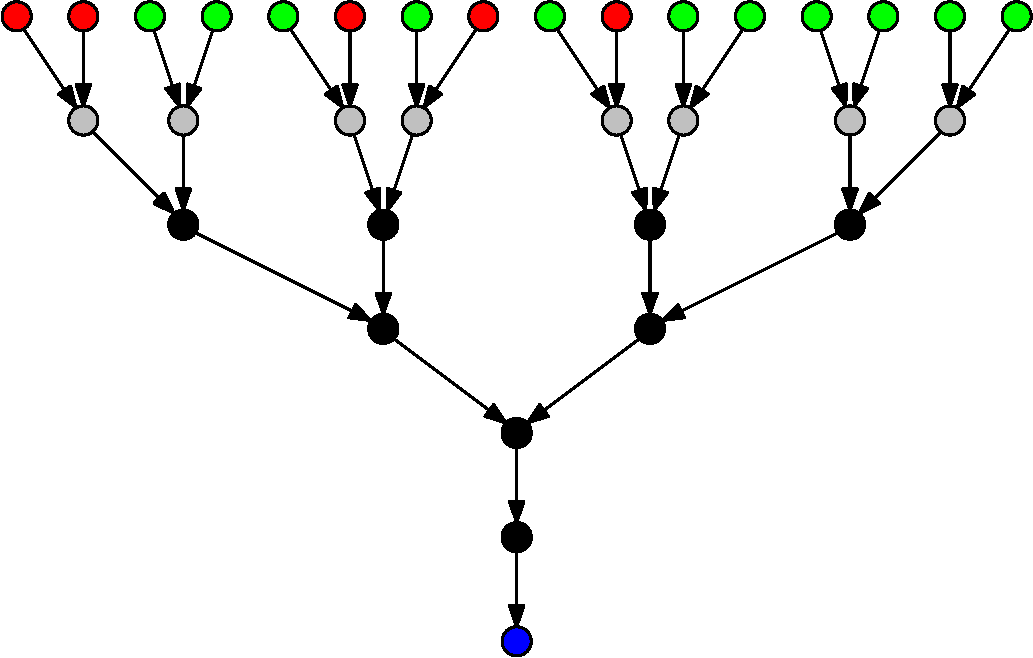
\includegraphics[scale=0.2]{topo-tree-evil-5-good-0-producer-gw}
  \caption{Small-scale binary tree topology}
  \label{fig:small-scale}
\end{figure}

% in 10 independent runs of each simulation, where we randomized position of the adversaries along the legitimate users.   In all runs, the total number of legitimate and malicious uses were fixed, meaning that when we increase number of attackers, we decrease the number of legitimate users.   

\subsubsection{Effectiveness of the three mitigation algorithms}

%The first set of experiments aims to evaluate reaction of the network and Interest flooding attack mitigation methods mechanisms under a moderate-level DDoS attack.
%For this purpose, we simulated four different network scenarios, in which all routers implements the same attack mitigation algorithm, either token bucket with per interface fairness, satisfaction-based Interest acceptance, or satisfaction-based pushback (Section~\ref{sec:design}).

Our goal is to compare the effectiveness of each mitigation method and quantify the percentage of Interests satisfied for all legitimate users while the network is under attack. For each mitigation algorithm, we perform ten independent simulation runs, where we randomly choose 7 client nodes to represent adversaries while the remaining 9 client nodes represent legitimate users. In each run we simulate a 10-minute attack window (total simulation time was 30 minutes, with attack starting at the 10-minute mark). We plot the minimum and maximum range for observed Interest satisfaction percentages for all legitimate users aggregated across the 10 simulation runs as a function of time for each mitigation algorithm in Fig.~\ref{fig:small-scale attack progress}. Token bucket with per-interface fair queuing performs the worst, while satisfaction-based pushback performs the best, with almost a 100\%  satisfied Interests for all legitimate users.

%A short and simplistic summary of the results is that the first two attack mitigation methods do not work at all, and the last two are working quite good.

\begin{figure}[]
  \centering
  \vspace{-.2cm}\hspace{-0.8cm}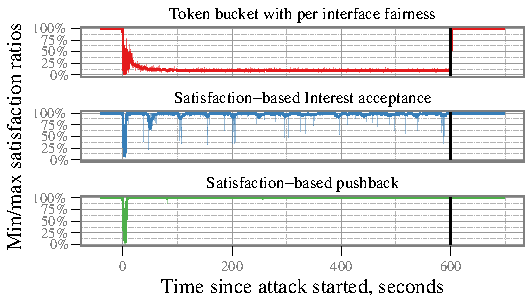
\includegraphics[scale=0.8]{paper-topo-tree/tree-good-0-producer-gw}
  \vspace{-.5cm}\caption{Interest satisfaction ratio as a function of time for binary-tree topology with 7 attackers and 9 legitimate users}
  \label{fig:small-scale attack progress}
\vspace{-.5cm}
\end{figure}

%\paragraph{\textbf{Simple token bucket}}

%{\color{red}Alex: should this discussion be removed or we still want to keep it (as it is referenced later and potentially before)}

%Let us take a deeper look on what is happening with the simple token bucket algorithm.
%Essentially, we observe an extremely successful denial of service attack, where attackers almost completely shut down legitimate users from the Data producer (using a relatively small amount of Interests, as token bucket restricts the number of forwarded Intersets!).
%This ``success'' can be explained using a simplistic example, illustrated on Fig.~\ref{fig:three router example}, where each router has only one token for Interest forwarding.
%In this example we assume that both the legitimate user and the adversary send Interests in about the same time.
%
%\begin{figure}[t]
%  \centering
%  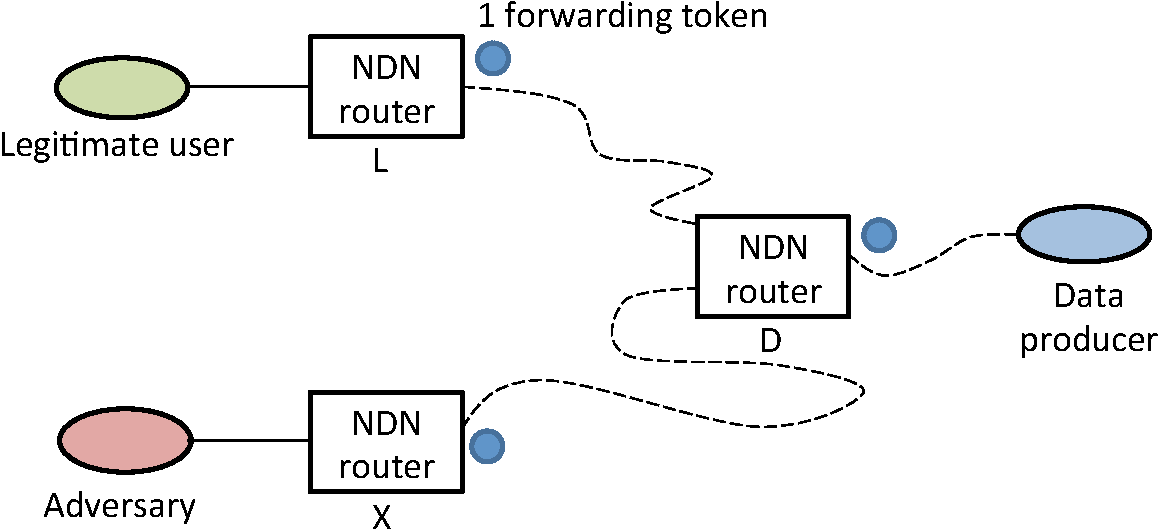
\includegraphics[scale=0.3]{physical-limits-sync-problem}
%  \caption{Three-router topology, with one legitimate and one malicious user}
%  \label{fig:three router example}
%\end{figure}
%
%Both router L and router X will forward the Interests, as both of them have a free token available.
%At router A, two cases are possible, either of Interests can arrive first, resulting in a quite different effects.
%When legitimate Interest arrives first, then there are no problem. 
%Router A will capture the token, forward the Interest, which will be quickly satisfied, releasing the token for future uses.
%In the mean time, malicious Interest will be dropped at router A, and router X will release the hold for the token in one second (i.e., after the maximum time Interests are admitted), enabling a new round of competition for router A's resources.
%
%In the case when malicious Interest is sent a little bit earlier, then router A will forward malicious Interests, dropping a legitimate one, and causing ``lock out'' for one second.
%In the instant when the token gets released at router X, an adversary is able to push new Interest towards router A, which may arrive in the exact time A's token gets released (assuming an idealistic environment).
%As a result, the adversary recaptures router A's token and extends the ``lock out'' for another second, denying service to the legitimate user without sending any massive numbers of Interests.

\paragraph{\textbf{Token bucket with per interface fairness}}

We observe a successful denial of service attack, where 40\% attackers succeed in significantly shutting down the remaining 60\% legitimate users - a mere 15\% of their Interests are satisfied by Data from the producer. Contrary to expectations, the 60\% legitimate users do not receive at least 60\% of network resources. As described in the previous section, the key limitation of this algorithm is that it still admits Interests from attackers, a good percentage of which traverse all the way to the data producer. Significantly reducing the number of Interests accepted from attackers is fundamental for improving the effectiveness of any mitigation algorithm. 

%The described problem arises from the clocking effect and can be solved in a number different ways.
%Augmenting token bucket algorithms with per-interface fair queueing allows us to eliminate the clocking effect. 
%That is, in the second case when router A releases the token after the first ``lock out'' period, it will immediately process previously enqueued Interests from the legitimate user.
%However, because the Interest time out (``lock out'' time) is most likely be larger than the time to actually fetch the Data, an adversary is still able to ``unfairly'' deny service to good guys.
%Ideally, if there are only 40\% of compromised users, the rest good users should get at least 60\% of network resources, which is not true as can be seen on Fig.~\ref{fig:small-scale attack progress}.
%We expect that reducing the maximum hold time for Interests (e.g., to an order of average RTT) would improve overall performance for legitimate users, with negative effect of requiring extra complexity for Intersets processing.

\paragraph{\textbf{Satisfaction-based Interest acceptance}}

The effectiveness of this algorithm stems from the fact that routers do not admit malicious Interests into the network, thereby ensuring availability of network resources for serving legitimate users. The observed periodic dips in the Interest satisfaction ratios of legitimate users in Fig.~\ref{fig:small-scale attack progress} is a direct result of Interest satisfaction rate statistics decaying with time. The 50-second period approximately corresponds to the selected exponential decaying parameter $\alpha=e^{−1.0/30.0}$, which decays statistics to $1/e$ of the initial value that ranges from 30~seconds to 50~seconds. 
%The primary reason that such minimum peaks exist is the fact that 
When Interests from attackers start to get readmitted, they cause degradation of statistics on routers close to the producer (i.e., routers that observe traffic mix from legitimate and malicious users). Consequently, this degradation reduces the probability of legitimate Interests getting through (see Section~\ref{sec:probabilistic}) until malicious Interests are ``pushed back'' to the edge.

%When routers more intelligently process incoming Interests (i.e., based on the incoming interface statistics), the Interest flooding attack becomes virtually ineffective.
%That is, malicious Interests are simply not getting admitted to the network, not being able to create much service disturbance for the legitimate users.

\paragraph{\textbf{Satisfaction-based pushback}}

This mitigation algorithm is able to effectively shut down attackers and ensure that almost all of the Interests from legitimate users are satisfied. 
%The only potential problem with the satisfaction-based pushback algorithm is that it features 
We observe a  sharp dip in the satisfaction ratio curve at the start of the attack.  It takes a few seconds for all routers to be fully aware of the attack, which happens when malicious Interests start to time out and explicit Interest limit announcements succeed in containing malicious Interests close to the attacker. Till then, the network for a short period of time (under 10~seconds for all simulation runs), fails to provide 100\% service for legitimate users. Once the malicious Interests are effectively shut down, all Interests from legitimate users are satisfied. Unlike the satisfaction-based Interest acceptance scenario, we do not observe any periodic dips in the satisfaction curve, as the pushback algorithm effectively guarantees that once an Interest is admitted, it will almost certainly be routed to the data producer.

\subsubsection{Network reaction with to varying number of attackers}

Our next goal is to study the effectiveness of our mitigation algorithms as a function of increasing adversaries in the network.
To this end, we vary the percentage of attackers in the topology from 6\% to over 50\%. Since the total number of end users in the topology is constant, as the number of attackers increases, the number of legitimate users decreases. All other parameters and experimental set-up are similar to the previous experiment. As before, for each mitigation algorithm, we perform ten independent simulation runs.
%The second set of conducted experiments was aimed to answer the question of the effect and quality of the Interest flooding attack mitigation algorithm under different attack volume.
%To do this, for each algorithm we varied the number of adversary nodes in the topology, keeping the total number of client nodes constant: 1 attacker and 15 legitimate users, 3 attackers and 13 legitimate users, etc.

%Since at this point the overall attack dynamics of all the attack mitigation algorithms is relatively clear, 
% In other words, each point captured in the box plot graph corresponds to 1-second averaged satisfaction ratio for a user in an individual simulation run.

\begin{figure}[htbp]
  \centering
  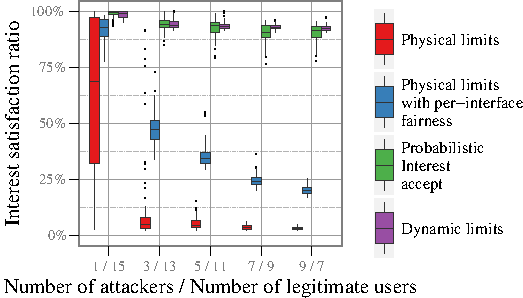
\includegraphics[scale=0.8]{paper-topo-tree/tree-good-0-producer-gw-avg-1-min}
  \vspace{-.6cm}\caption{Average Interest satisfaction ratios for the first minute of the experiment as a function of increasing attackers in the network}\vspace{-.1cm}
  \label{fig:small-scale-topo boxplot}
\end{figure}

In Fig.\ref{fig:small-scale-topo boxplot} we present  the Interest satisfaction ratio for legitimate users aggregated over the 10 simulation runs for the first minute of the attack. The results are as expected---for all three mitigation algorithms, as the percentage of attackers in the network increases, the lower is the Interest satisfaction ratio for legitimate users.
In the case of token bucket with per-interface fairness algorithm, just 3 attackers can halve the quality of service for the remaining 13 legitimate users. While both intelligent attack mitigation algorithms also show a decline in service quality as the percentage of attackers increases, this decline is much more gradual. In the case of satisfaction-based pushback algorithm, over 90\% of Interests from legitimate users are satisfied even when over 50\% of the users are malicious.  
 


% \begin{figure}[htbp]
%   \centering
%   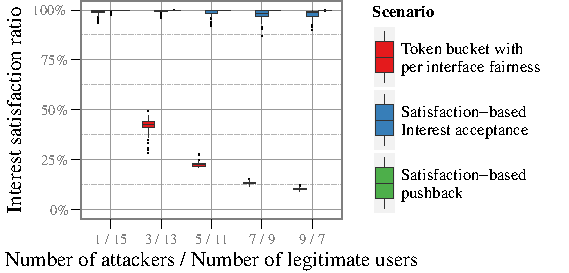
\includegraphics[scale=0.9]{tree-topo-var-evils-max-consumers-30mins/tree-good-0-producer-gw-avg-1-min-after-1-min}
%   \caption{Average consumer Interest satisfaction ratios (second minute)}
%   \label{fig:small-scale-topo 2}
% \end{figure}


%%% Local Variables: 
%%% mode: latex
%%% TeX-master: "paper"
%%% End: 

\subsection{Large scale simulations}
\label{sec:largescale}

To check validity of the small-scale experiment results, we performed a larger-scale evaluation based on a modified version of Rocketfuel AT\&T topology~\cite{rocketfuel}.
In order to approximate the general structure of the Internet,
% (scale-free structure, customer-provider, and peer-to-peer relations)
we extracted the largest connected component of 562 nodes from the original topology and separated nodes in three categories: clients, gateways, and backbones.
All nodes with degrees one, two, and three became clients (344 red nodes on Fig.~\ref{fig:large-scale}), all nodes that are directly connected to clients became gateways (109 green nodes), and the rest became backbones (109 blue nodes).
(To ensure that paths in the topology are ``valley-free,'' we augmented the topology with necessary backbone-to-backbone links.)
After categorizing the nodes, we randomly assigned bandwidths and link delays based on link types (see Table~\ref{tab:large-scale}).

\begin{figure}[htbp]
  \centering
  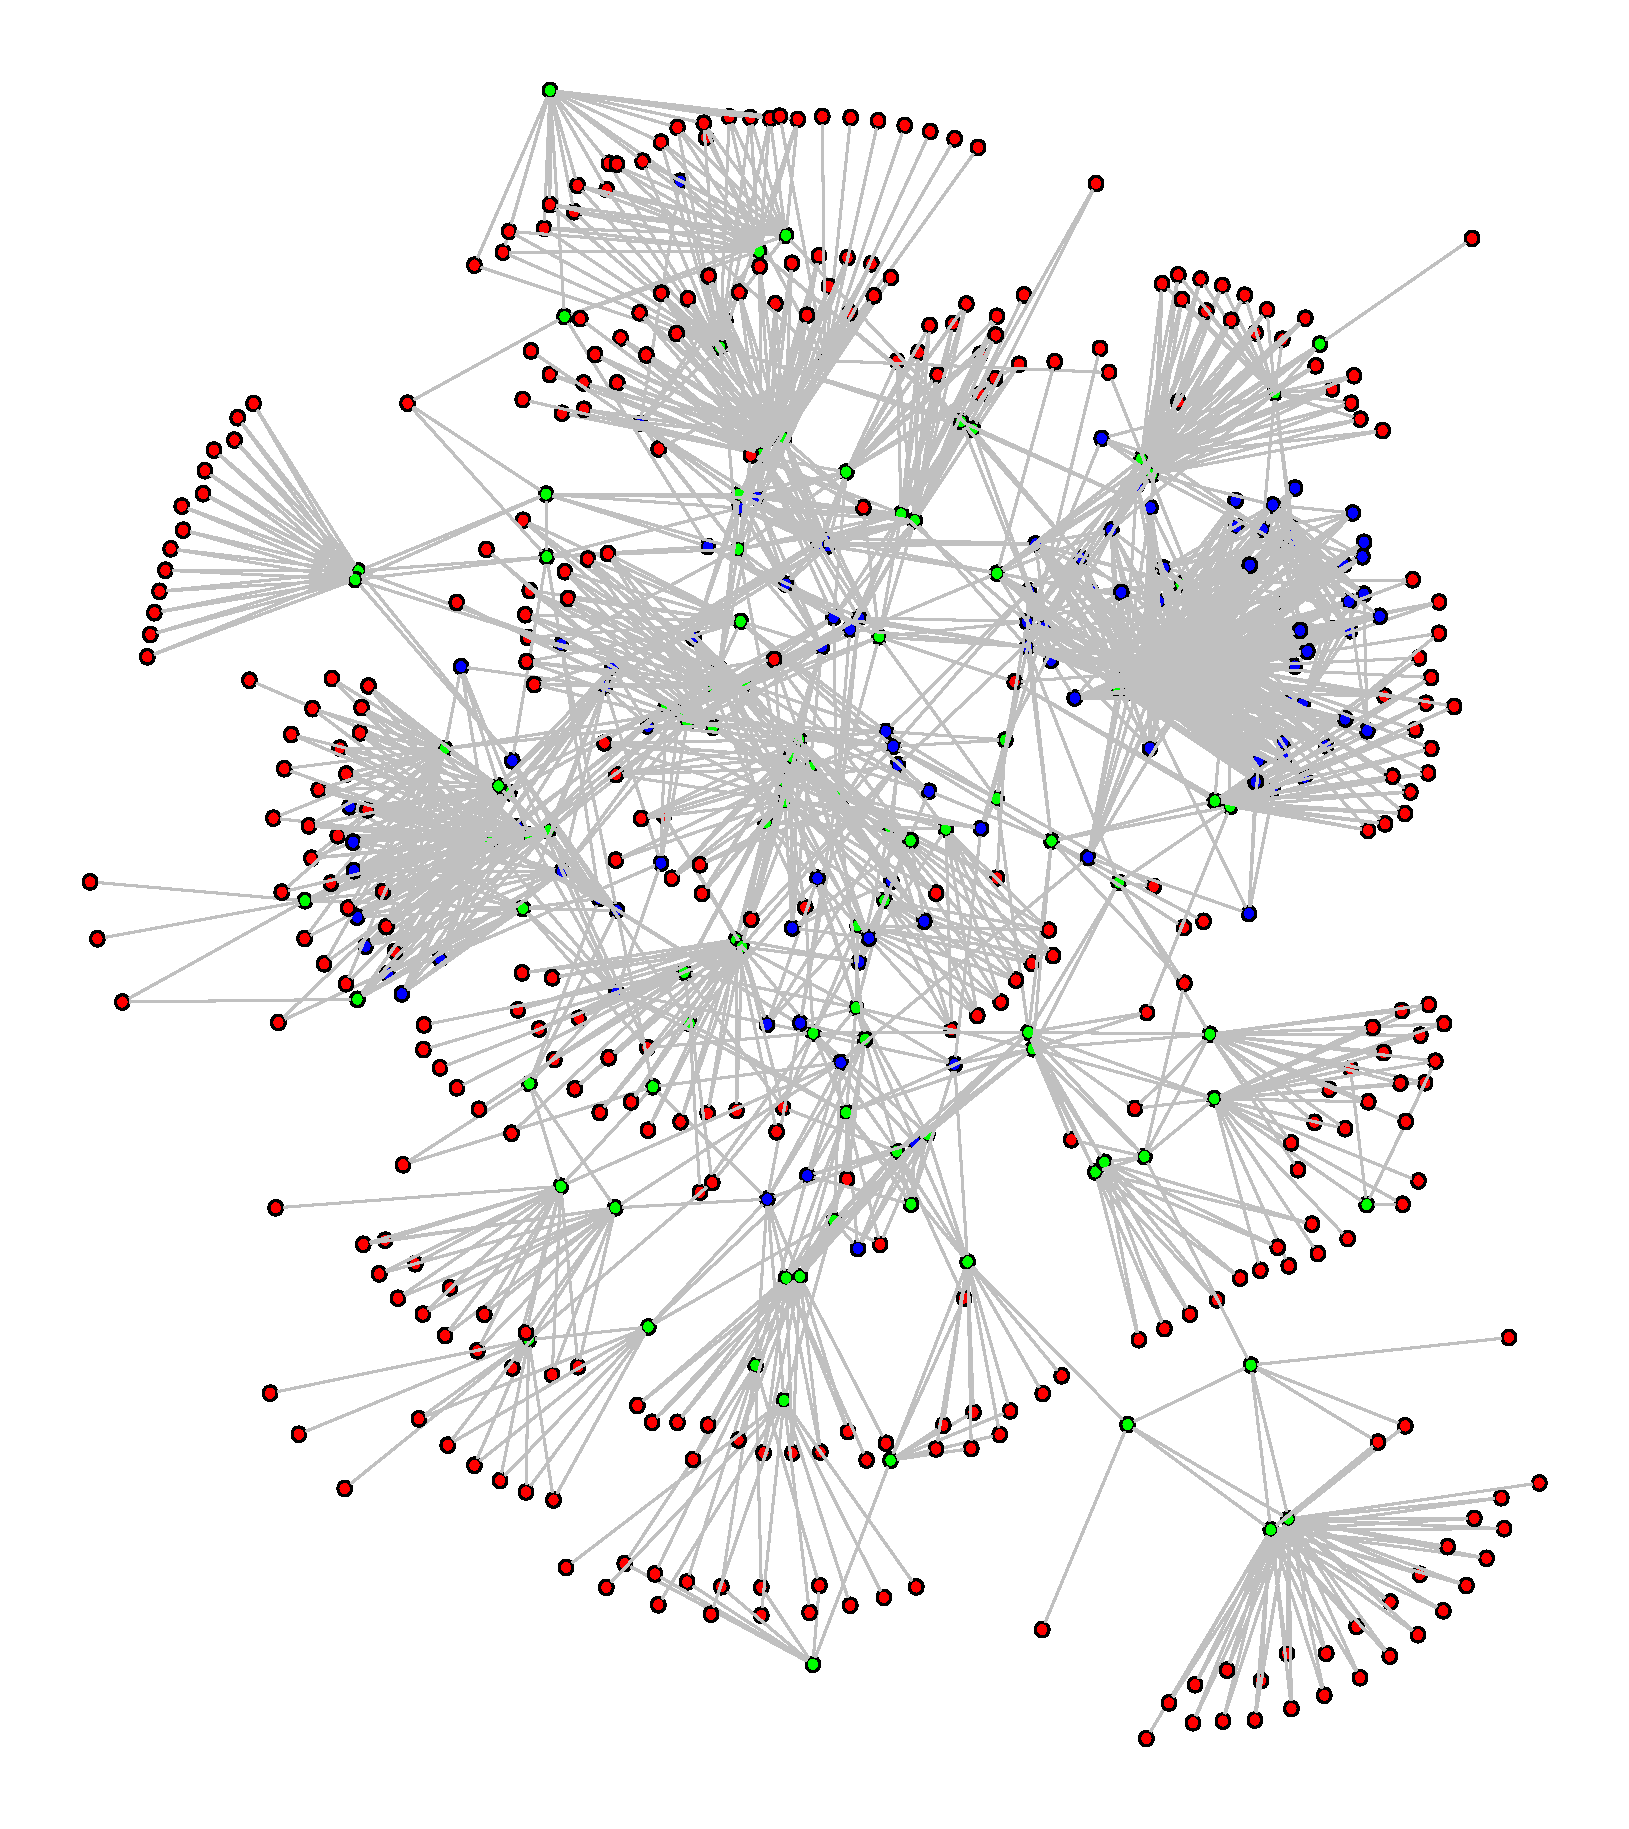
\includegraphics[scale=0.26,angle=90]{7018-r0}
  \caption{Internet-like topology: 344 client routers (red), 109 gateway routers (green), 109 backbone routers (blue)}
  \label{fig:large-scale-topo}
\end{figure}

\begin{table}[htbp]
\centering
\caption{Large-scale topology parameters}
\label{tab:large-scale}
\begin{tabular}{|l||c|c||c|c|}
  \hline
  \multirow{2}{*}{\bf Link type} &  \multicolumn{2}{|c||}{\bf Delay} &  \multicolumn{2}{|c|}{\bf Bandwidth} \tabularnewline
  \cline{2-5}
                        &  Min & Max                       &  Min & Max \tabularnewline
  \hline \hline
  Backbone--Backbone    & 5~ms & 10~ms   & 40~Mbps & 100~Mbps \tabularnewline
  \hline
  Gateway--Backbone,    & \multirow{2}{*}{5~ms} & \multirow{2}{*}{10~ms}   
                        & \multirow{2}{*}{10~Mbps} & \multirow{2}{*}{20~Mbps} \tabularnewline
  Gateway--Gateway      & & & & \\
  \hline
  Client--Gateway       & 10~ms & 70~ms   & 1~Mbps  & 3~Mbps \\
  \hline

\end{tabular}
\end{table}

In an Internet-like topology, the location of the Data producer plays the key part in his ability to sustain flooding attack.
That is, if the producer has limited network capacity (a personal blog located hosted on a client node), then he will be a really easy target for the attack.
On the other extreme, when the producer is located at the backbone (Google or Amamzon), then the attack would have a hard time to degrade service, as a lot of legitimate users would not even share paths with attackers.
To evaluate a balanced network scenario, we placed the Data producer at the gateway node, which randomly picked for each simulation run.
Similarly to the first set of small-scale evaluations, we fixed the number of malicious nodes at approximately 40\% level (140 out of 344 client nodes in the topology), while randomly varied which locations of compromised nodes.

% The results for all attack mitigation algorithms and all runs are aggregated in Fig.~\ref{fig:small-scale attack progress}, where Y-axis represents a minimum and maximum range for observed Interest satisfaction percentages among all nodes and all simulation runs.
% A short and simplistic summary of the results is that the first two attack mitigation methods do not work at all, and the last two are working quite good.

The evaluation results,\footnote{Note that for larger-scale experiments we reduced attack window to 15~minutes} summarized in Fig.~\ref{fig:large-scale}, show that for both physical limits algorithms and dynamic limits algorithm the performance is about the same as in small-scale evaluations (Fig.~\ref{fig:small-scale}), but with larger variations of minimum and maximum instantaneous satisfaction rates.

\begin{figure}[tbh]
 \centering
 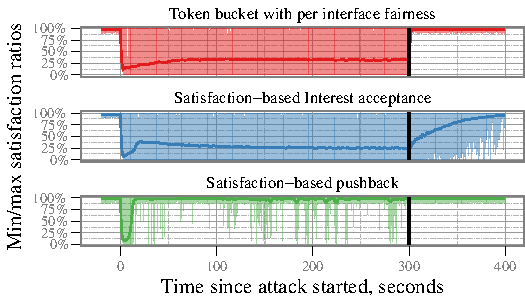
\includegraphics[scale=1]{topo-7018-gw-15mins-new/7018-r0-good-0-producer-gw}
 \caption{Satisfaction ratio dynamics during the attack (30\% attackers)}
 % producer on a gateway node
 \label{fig:large-scale}
\end{figure}

At the same time, the probabilistic method completely failed to provide an adequate protection against the Interest flooding attack, and in addition degraded service for the legitimate users after the attack finished.
The main reason for the failure was already explained in Section~\ref{sec:probabilistic}.
That is, if the number of hops between legitimate users and the Data producer is large (15 on average in the simulated topology) uncoordinated probabilistic Interest drops result in minuscule probability for good Interests to reach the Data producer during an ongoing attack, resulting in negative Interests satisfaction ratio statistics.
This also explains why until the statistics ages out, not all legitimate users can get satisfy all of their Interests.

In summary, in all of the simulated topologies, the dynamic limits algorithm restricts malicious traffic from even entering the network.
The only short periods of time when malicious Interests are getting admitted to the network is when routers have either no prior knowledge about per-interface satisfaction ratios (the initial period of the attack) or such knowledge becomes stale (statistics decaying during the attack).
As soon as the knowledge is obtained or refreshed, the service for legitimate users returns to norm.


% Alex: Anything else here?

% Alex: I also experimented with placing producer at the backbone, getting slightly better results for all algorithms.  Though I'm not sure there is any value to put those results in the paper


%%% Local Variables: 
%%% mode: latex
%%% TeX-master: "paper"
%%% End: 


% \subsection{Simulation versus Emulation}
\label{sec:simemu}
Before committing significant efforts into simulation-based implementation of designed defensive techniques it was necessary to confirm that ndnSIM has close performance characteristics to the reference NDN implementation - Project CCNx. This will guarantee that evaluation results derived from simulations will be meaningful in real NDN world.

To achieve this goal a comparison of Project CCNx software and ndnSIM software was performed under small scale Interest flooding attack. DETER Testbed was used as emulation tool for CCNx evaluation. Using it we were able to setup non-virtualized Ubuntu nodes running CCNx 0.6.0 software connected in a binary tree topology with 4 leaves and 1 root node. A number of applications running on top of CCNx have been developed, namely:
\begin{itemize}
\item{Producer application serves 1KB data packets under a known for the attacker name prefix}
\item{Legitimate client application requests 5KB of data per second from the producer}
\item{Attacker application tries to fill the channel of the producer by sending 500 Interest packets per second}
\end{itemize} 

In this emulation scenario producer application occupied a root node, legitimate clients occupied all even leaves and attacker applications were put on all odd leaves. With 100kb links with 40ms delay such setup leads to no congestion during the period when attackers are turned off and congestion when they are turned on (seconds 60-90). Exactly the same scenario was replicated for ndnSIM evaluation, however, we had to adjust the sending rate of attacker application in order to produce the same amount of congestion in the network. Sending rates are compared in Figure~\ref{fig:simemupower}. To achieve the identical slope and height of sending rate of evil Interests by attacker nodes we had to reduce sending rate of simulation-based attacker application by 30\%. The most likely reason for that is the overhead of Java virtual machine and operating system itself during the emulation of CCNx that results in eventual 30\% slower Interest transmission.  

Once we achieved the same characteristics of Interest flooding attack we were able to compare data packet losses by legitimate clients. Figure~\ref{fig:simemuperf} shows the cumulative received data by legitimate consumers in emulation and simulation experiments. NdnSIM performs worse due to its more deterministic nature, while the effects of UDP protocol usage, operating system process scheduling, and other kernel level operations on packet queues provide more randomness and a better intermixing of bad and good traffic which gives a slightly better performance. To summarize, we can use ndnSIM for our evaluations and real world performance is likely to be even better than our evaluation results.

\begin{figure}[htpb]
  \centering
  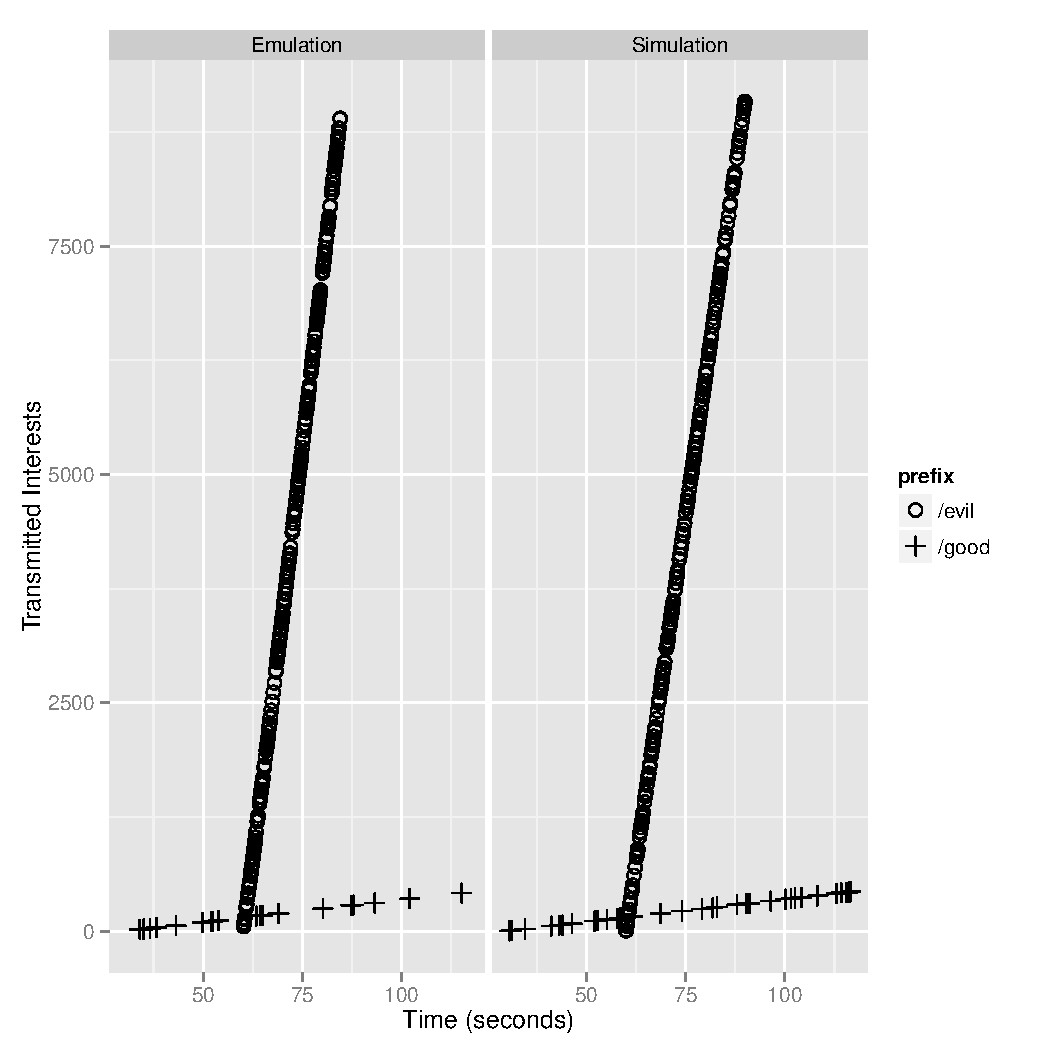
\includegraphics[scale=0.5]{figures/sim-emu-power.pdf}
  \caption{Strength of Interest flooding attack}
  \label{fig:simemupower}
\end{figure}

\begin{figure}[htpb]
  \centering
  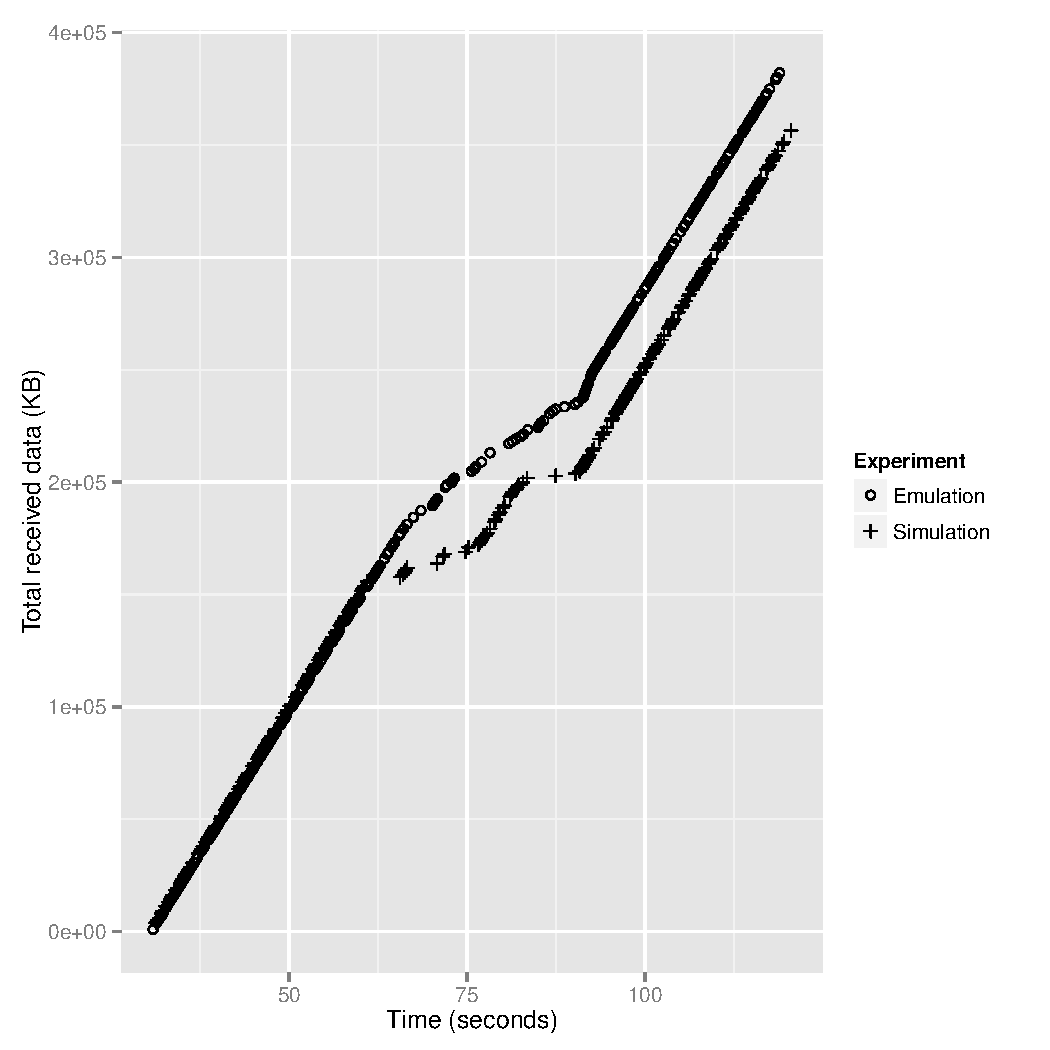
\includegraphics[scale=0.5]{figures/sim-emu-performance.pdf}
  \caption{Data retrieval by legitimate clients}
  \label{fig:simemuperf}
\end{figure}



%%% Local Variables: 
%%% mode: latex
%%% TeX-master: "paper"
%%% End: 
